% !TEX root = ../OT4ML.tex

\chapter{Generative Models via Transportation}
\index{generative model}% strictindex
\label{sec-generative-models-transportation}

The preceding gradient-flow calculus is variational. Modern machine-learning models often use the same transportation language more broadly: one may prescribe an interpolation and regress its velocity, fit a one-step generator to a descent field, or view network depth as a continuous transport of token measures. The examples below separate what is genuinely a Wasserstein gradient flow from what is a transportation dynamics with a useful geometric interpretation.
\index{Wasserstein!gradient}% strictindex
\index{gradient!flow}% strictindex
\index{Wasserstein!gradient flow}% strictindex
\index{token measure}% strictindex

\section{Generative Models via Flow Matching}
\index{flow!matching}% strictindex
\index{generative model}% strictindex

Flow matching constructs a generative map by learning the velocity field of an interpolation. The key computational insight is that a constrained continuity-equation problem can be trained by an unconstrained regression.
\index{velocity field}% strictindex
\index{continuity equation}% strictindex
\index{flow!matching}% strictindex

Generative models aim to build a transportation map $T$ between a reference distribution $\alpha$ (typically an isotropic Gaussian) and the target data distribution $\beta$. Since such reference measures are non-atomic, a measurable map with $T_\sharp\alpha=\beta$ exists on standard Borel spaces, for instance by identifying both probability spaces with the unit interval and using a quantile-type rearrangement. This abstract existence statement is much weaker than having an explicit and numerically stable construction of $T$.
\index{reference!distribution}% strictindex
\index{reference!measure}% strictindex
\index{generative model}% strictindex
%
Optimal transport is one approach to achieving this, but it is computationally expensive and raises questions about how to estimate it from samples. A different route is to prescribe an interpolation between noise and data, learn its velocity, and obtain $T$ by integrating a time-dependent vector field $v_t$. This point of view sits at the meeting point of two literatures, surveyed from a transport perspective in~\cite{Peyre2026OptimalDiffusionTransports}. The diffusion branch builds on score matching~\cite{Hyvarinen2005ScoreMatching}, denoising score matching~\cite{Vincent2011DenoisingScoreMatching}, nonequilibrium noising chains~\cite{SohlDickstein2015DeepUnsupervised}, denoising diffusion probabilistic models~\cite{Ho2020DDPM}, score-based generative modeling~\cite{Song2019ScoreMatchingGenerative}, and the continuous-time score-SDE/probability-flow formulation~\cite{Song2021ScoreSDE}. The deterministic regression branch was introduced, essentially in parallel, under three closely related names: flow matching~\cite{Lipman2022FlowMatching}, rectified flow~\cite{Liu2023RectifiedFlow}, and stochastic interpolants~\cite{Albergo2025StochasticInterpolants}. In all three cases, the computational object is a velocity field whose regression loss avoids simulating the learned ODE during training.
\index{denoising diffusion probabilistic model}% strictindex
\index{score-SDE}% strictindex
\index{probability-flow ODE}% strictindex
\index{score-based generative modeling}% strictindex
\index{velocity field}% strictindex
\index{integral probability metric}% strictindex
\index{flow!matching}% strictindex
\index{time-dependent vector field}% strictindex
\index{denoising score matching}% strictindex
\index{stochastic!interpolant}% strictindex
\index{regression loss}% strictindex
\index{flow!rectified}% strictindex
\index{flow!matching}% strictindex
%
This vector field $v_t$ is obtained by constructing an interpolation $\alpha_t$ and then finding $v_t$ using the least-squares formula~\eqref{eq:least-square-field-explicit}. As we will explain, for a specific class of interpolation (obtained by a parametric push-forward), this $v_t$ can be obtained by avoiding explicitly inverting a Laplacian and instead computing a simple conditional expectation. This conditional expectation can itself be estimated by solving another least-squares problem, but this time unconstrained, making the estimation feasible from finite samples of $\alpha$ and $\beta$.
\index{conditional!expectation}% strictindex
\index{push-forward}% strictindex

\paragraph{Stochastic interpolant.}
\index{stochastic!interpolant}% strictindex


We assume that $\alpha_t$ is defined via a ``projection'' (in a loose sense) of a latent distribution $\pi \in \Pp(\RR^{d'})$, using an operator $P_t : \RR^{d'} \to \RR^d$ where $d' \gg d$, i.e.
\begin{equation}\label{eq:interp-coupling}
	\forall t \in [0,1], \quad \alpha_t := (P_t)_\sharp \pi.
\end{equation}
The basic two-endpoint construction already covers most flow-matching paths used in practice.

\begin{example}[Linear two-endpoint stochastic interpolants]
	Set $d'=2d$, write $(x,y)\in\RR^d\times\RR^d$, and choose $P_0(x,y)=x$ and $P_1(x,y)=y$. If $\pi$ has marginals $(\alpha_0,\alpha_1)$, then $\alpha_t=(P_t)_\sharp\pi$ interpolates between the two endpoint laws. The simplest choices are the independent coupling $\pi=\alpha_0\otimes\alpha_1$ and the straight path
	\[
		P_t(x,y)=(1-t)x+ty.
	\]
	With this linear path and an arbitrary coupling $\pi$, the regression below is the common core of flow matching and rectified flow: Lipman et al. emphasize conditional probability paths and simulation-free training of continuous normalizing flows, while rectified flow emphasizes straight couplings, reflow, and the possibility of reducing transport costs and discretization error~\cite{Lipman2022FlowMatching,Liu2023RectifiedFlow}.

	More complex constructions are possible when sampling from $\pi$ remains simple; stochastic interpolants add latent variables or noise, connecting deterministic flows, probability-flow ODEs and diffusion SDEs~\cite{Albergo2025StochasticInterpolants}.
\end{example}
\index{continuous normalizing flow}% strictindex
\index{reflow}% strictindex
\index{discretization error}% strictindex
\index{latent variable}% strictindex
\index{conditional probability}% strictindex
\index{probability-flow ODE}% strictindex
\index{normalizing flow}% strictindex
\index{probability path}% strictindex
\index{integral probability metric}% strictindex
\index{flow!matching}% strictindex
\index{flow!rectified}% strictindex
\index{flow!probability ODE}% strictindex
\index{probabilistic coupling}% strictindex
\index{stochastic!interpolant}% strictindex
\index{probability path}% strictindex
\index{trivial coupling}% strictindex
\index{flow!rectified}% strictindex
\index{flow!matching}% strictindex

If $\pi = \alpha \otimes \beta$ and $\alpha = \frac{1}{n} \sum_i \delta_{x_i}$, $\beta = \frac{1}{m} \sum_j \delta_{y_j}$, then $\alpha_t$ consists of $n \times m$ Dirac masses
\index{Dirac mass}% strictindex
\begin{equation*}
    \alpha_t = \frac{1}{nm} \sum_{i,j} \delta_{P_t(x_i,y_j)}.
\end{equation*}
If $\pi = (\Id, T)_\sharp \alpha$ is a Brenier-type coupling, then $\alpha_t = ((1-t)\Id + tT)_\sharp \alpha$ is the so-called McCann OT interpolation.

\begin{figure}[H]
\centering
\begin{tabular}{@{}ccc@{}}
\small product pairing & \small OT pairing & \small curved bridge \\[-.15em]
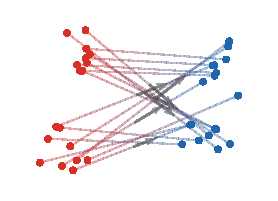
\includegraphics[width=.30\linewidth]{figures/generative-flow-matching-interpolants/product-linear.pdf} &
\index{flow!matching}% strictindex

\includegraphics[width=.30\linewidth]{figures/generative-flow-matching-interpolants/ot-linear.pdf} &
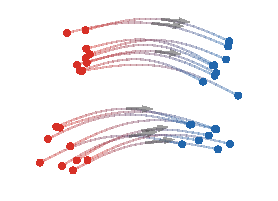
\includegraphics[width=.30\linewidth]{figures/generative-flow-matching-interpolants/curved-bridge.pdf}
\end{tabular}
\caption{Flow matching interpolants between the same empirical source and target measures. A product-style random pairing produces crossing paths, an OT pairing gives direct displacement rays, and a curved bridge changes the path geometry while keeping the same endpoints. Gray arrows mark representative midpoint velocities $\partial_tP_t$.}
\index{flow!matching}% strictindex
\label{fig:generative-flow-matching-interpolants}
\end{figure}

\paragraph{Flow matching formula.}
\index{flow!matching}% strictindex

This interpolation is not directly useful for sampling from $\beta$, but it can be used to define a flow field $v_t$ so that the Eulerian advection equation~\eqref{eq:eulerian-advection} holds.
%
This flow field is computed by solving an unconstrained least-squares problem, or equivalently, it is a conditional expectation.
\index{conditional!expectation}% strictindex

\begin{prop}[Flow matching vector field]\label{prop-flow-matching-vector-field}
\index{flow!matching}% strictindex
	For each fixed $t$, assume $\partial_tP_t\in L^2(\pi;\RR^d)$. The solution of the flow-matching problem over measurable fields $v_t:\RR^d\to\RR^d$
\index{assignment problem}% strictindex
\index{flow!matching}% strictindex
	\begin{equation}
		\min_{v_t} \int_{\RR^{d'}} \norm{v_t(P_t(u)) - [\partial_t P_t](u)}^2 \, \d\pi(u). \label{eq:flow-matching}
	\end{equation}
	Equivalently, the minimizer is characterized $\alpha_t$-almost everywhere by the conditional expectation
\index{conditional!expectation}% strictindex
	\begin{equation}\label{eq:flow-match-conditional}
		v_t(z) = \EE_{u \sim \pi} \big( [\partial_t P_t](u) \, \big| \, z = P_t(u) \big).
	\end{equation}
	Then the pair $(\alpha_t,v_t)$ satisfies the continuity equation~\eqref{eq:eulerian-advection}.
\index{continuity equation}% strictindex
\end{prop}

\begin{proof}
	We first recall the two equivalent ways of writing the interpolated measure. Formally, one may write
	\[
		\alpha_t(z)=\int_{\RR^{d'}}\delta(z-P_t(u))\,\d\pi(u),
	\]
	while the rigorous meaning is that, for every smooth test function $\varphi$,
	\begin{equation}\label{eq:flow-matching-pushforward-test}
\index{push-forward}% strictindex
		\int_{\RR^d}\varphi(z)\,\d\alpha_t(z)
		=
		\int_{\RR^{d'}}\varphi(P_t(u))\,\d\pi(u).
	\end{equation}
	The minimizer in~\eqref{eq:flow-matching} is the orthogonal projection in $L^2(\pi;\RR^d)$ of the latent velocity $\partial_tP_t(u)$ onto the closed subspace of functions that depend on $u$ only through $P_t(u)$. This projection is the conditional expectation~\eqref{eq:flow-match-conditional}. Formally, this can be read as
\index{conditional!expectation}% strictindex
\index{flow!matching}% strictindex
	\[
		v_t(z)=\frac{1}{\alpha_t(z)}
		\int_{\RR^{d'}}\delta(z-P_t(u))[\partial_tP_t](u)\,\d\pi(u),
	\]
	and rigorously it means that, for every smooth test vector field $m$,
	\begin{equation}\label{eq:v_t}
		\int \dotp{m(z)}{v_t(z)} \, \d\alpha_t(z)
		=
		\int \dotp{m(P_t(u))}{[\partial_t P_t](u)} \, \d\pi(u).
	\end{equation}

	We now prove that this field transports the curve $(\alpha_t)_t$. The weak form of
	$\partial_t\alpha_t+\diverg(\alpha_t v_t)=0$ is that, for every smooth scalar test function $\varphi$,
	\begin{equation}\label{eq:flow-matching-weak-target}
		\frac{\d}{\d t}\int\varphi(z)\,\d\alpha_t(z)
		-
		\int\dotp{v_t(z)}{\nabla\varphi(z)}\,\d\alpha_t(z)
		=0.
	\end{equation}
	Using~\eqref{eq:flow-matching-pushforward-test} and differentiating under the integral sign gives
\index{push-forward}% strictindex
\index{flow!matching}% strictindex
	\begin{equation}\label{eq:flow-matching-test-derivative}
		\frac{\d}{\d t}\int \varphi(z)\d\alpha_t(z)
		=
		\int \dotp{\nabla\varphi(P_t(u))}{[\partial_t P_t](u)}\d\pi(u).
	\end{equation}
	On the other hand, applying~\eqref{eq:v_t} with $m=\nabla\varphi$ gives
	\begin{equation}\label{eq:flow-matching-velocity-test}
		\int\dotp{v_t(z)}{\nabla\varphi(z)}\,\d\alpha_t(z)
		=
		\int \dotp{\nabla\varphi(P_t(u))}{[\partial_t P_t](u)}\d\pi(u).
	\end{equation}
	Comparing~\eqref{eq:flow-matching-test-derivative} and~\eqref{eq:flow-matching-velocity-test} yields~\eqref{eq:flow-matching-weak-target}, which is the desired continuity equation.
\index{continuity equation}% strictindex
\index{flow!matching}% strictindex
\end{proof}

The conditional expectation in~\eqref{eq:flow-match-conditional} has a simple measure-theoretic meaning. Let $\alpha_t=(P_t)_\sharp\pi$ and define the vector-valued measure $m_t$ on $\RR^d$ by
\[
	\int_{\RR^d}\dotp{\psi(z)}{\d m_t(z)}
	\eqdef
	\int_{\RR^{d'}}\dotp{\psi(P_t(u))}{[\partial_tP_t](u)}\d\pi(u)
\]
for every bounded continuous vector field $\psi$. Since $\alpha_t(A)=0$ implies $\pi(P_t^{-1}(A))=0$, one has $m_t\ll\alpha_t$. The Radon--Nikodym decomposition of $m_t$ with respect to $\alpha_t$ is therefore
\[
	\d m_t(z)=v_t(z)\d\alpha_t(z),
	\qquad
	v_t=\frac{\d m_t}{\d\alpha_t}.
\]
In the language of Lebesgue decomposition, the flux measure $m_t$ has only an absolutely continuous part with respect to $\alpha_t$ and no singular part; the conditional expectation is precisely this density.
Equivalently, disintegrating $\pi$ with respect to the map $P_t$ gives $\pi(\d u)=\pi_{t,z}(\d u)\alpha_t(\d z)$, where $\pi_{t,z}$ is supported on the fiber $\{u\,:\,P_t(u)=z\}$, and
\[
	v_t(z)=\int_{\{P_t(u)=z\}}[\partial_tP_t](u)\d\pi_{t,z}(u).
\]
Thus the solution of \eqref{eq:flow-matching} is the conditional expectation of the velocities $\partial_t P_t$: intuitively, $v_t(z)$ is the average velocity of all trajectories passing through $z$.
\index{conditional!expectation}% strictindex
\index{Radon-Nikodym derivative}% strictindex
\index{disintegration}% strictindex
%
Numerically, $(x,t) \to v_t(x)$ can be parameterized by a neural network (e.g., a U-Net for vision tasks) and estimated using stochastic gradient descent on the objective in \eqref{eq:flow-matching}.
\index{stochastic!gradient}% strictindex
\index{flow!matching}% strictindex
%

\begin{alg}[Flow matching regression and sampling]\label{alg:flow-matching-regression}
\index{flow!matching}% strictindex
\textbf{Input:} Interpolant $P_t(u)$, training source $u\sim\pi$, parametrized field $v_\theta(t,z)$, training steps $N$.

\textbf{Output:} Learned sampler $X_0\mapsto X_1$.

\textbf{Training:}

\textbf{For} $q=1,\ldots,N$ \textbf{do}:
\begin{algblock}
\textbf{Draw} $t_q\sim\mathrm{Unif}(0,1)$ and $u_q\sim\pi$.

\textbf{Set} $z_q=P_{t_q}(u_q)$ and $w_q=\partial_tP_t(u_q)|_{t=t_q}$.

\textbf{Update} $\theta$ by one stochastic-gradient step on \(\norm{v_\theta(t_q,z_q)-w_q}^2.\)

\end{algblock}

\textbf{Sampling:}

\textbf{Draw} $X_0\sim\alpha_0$.

\textbf{Integrate}
\(\dot X_t=v_\theta(t,X_t), \qquad t\in[0,1].\)

\textbf{Return} $X_1$.
\end{alg}

For the exact field $v_t$, integrating the ODE $\dot{x}=v_t(x)$ defines a transport map $T_t$. If $v_t$ is regular enough, or more generally if the continuity equation has a unique solution for this velocity, then $(T_t)_\sharp\alpha_0=\alpha_t$. Thus the same interpolation as~\eqref{eq:interp-coupling} is represented by a deterministic flow rather than by the original coupling.
\index{transport map}% strictindex
\index{continuity equation}% strictindex
The sampling procedure consists in first drawing $X_0 \sim \alpha$, and then integrating the ODE $\dot{X}_t = v_t(X_t)$ starting with $X_{t=0} = X_0$.
In the ideal exact-field limit, the resulting $X_{t=1}$ is distributed according to $\alpha_1 = \beta$.

\paragraph{Connection with diffusion models.}
\index{diffusion model}% strictindex

In the special case where $P_t(x,y)=(1-t)x+ty$ is a linear interpolation and $\pi = \alpha \otimes \beta$, the curve $\alpha_t$ is a convolution of rescaled versions of $\alpha_0$ and $\alpha_1$. The flow-matching problem~\eqref{eq:flow-matching} becomes
\index{assignment problem}% strictindex
\index{flow!matching}% strictindex
\[
    \min_{(v_t)_t} \int_{\RR^{d} \times \RR^d} \norm{v_t( (1-t)x+t y ) - (y-x) }^2 \, \d\alpha_0(x) \d\alpha_1(y).
\]
When one endpoint is an isotropic Gaussian, this construction is closely related to the probability-flow formulation of diffusion models, up to the usual change of time parametrization~\cite{Song2021ScoreSDE}. This is why flow matching can be viewed both as a deterministic alternative to diffusion training and as a common language for diffusion paths, OT-inspired paths, and rectified paths~\cite{Lipman2022FlowMatching,Liu2023RectifiedFlow,Albergo2025StochasticInterpolants}. The next two propositions are written in the noising direction, from a data law $\alpha$ to a Gaussian; reversing time gives the corresponding sampling flow. They also give an explicit closed form for $v_t$ and show that it is a gradient field.
\index{probability-flow ODE}% strictindex
\index{integral probability metric}% strictindex
\index{diffusion model}% strictindex
\index{flow!matching}% strictindex
%
In this setting, $v_t$ is also the solution of the constrained least-squares problem~\eqref{eq:least-square-field-explicit}. The regression~\eqref{eq:flow-matching} is computationally simpler because the continuity equation has already been enforced by the chosen interpolant.
\index{continuity equation}% strictindex
%
To prove this, we rely on Tweedie's formula, which expresses the optimal Gaussian denoiser through the score, i.e. the gradient of the log-density.
\index{Gaussian denoiser}% strictindex
\index{score function}% strictindex
\index{Tweedie identity}% strictindex

\begin{proposition}[Tweedie identity]\label{prop:Tweedie}
Let $W$ be a random vector in $\RR^{d}$ with density $\beta$.
For $\sigma>0$, observe
\[
Z \;=\; W + \sigma\,\varepsilon,
\quad\text{where } \varepsilon \sim \Gaussian(0,I_{d})
\text{ is independent of } W .
\]
Denote by
\[
	\beta_\sigma \;=\; \beta * \Gaussian\bigl(0,\sigma^{2}I_{d}\bigr)
\]
the density of $Z$.
Then
\[
\EE\bigl[\,W \mid Z=z\bigr]
      \;=\; z \;+\;\sigma^{2}\,\nabla \log \beta_\sigma(z)
\qquad\text{for all } z \in \RR^{d}.
\]
\end{proposition}

\begin{proof}
Bayes' rule gives the conditional density
$
p_{W|Z}(w\mid z)
= \dfrac{\beta(w)\,\varphi_\sigma(z-w)}{\beta_\sigma(z)}
$
with $\varphi_\sigma$ the $\Gaussian(0,\sigma^{2}I_{d})$ density.
Hence
\[
\EE[W\mid Z=z]
= \frac{1}{\beta_\sigma(z)}
      \int_{\RR^{d}} w\,
             \beta(w)\,\varphi_\sigma(z-w)\,\d w .
\]
Differentiating the Gaussian convolution under the integral sign and using
$
\nabla_z\varphi_\sigma(z-w)
     = -\sigma^{-2}(z-w)\,\varphi_\sigma(z-w)
$
yields
\[
\nabla_z\beta_\sigma(z)
= \int \beta(w)\,\nabla_z\varphi_\sigma(z-w)\,\d w
= -\sigma^{-2}\Bigl(z-\EE[W\mid Z=z]\Bigr)\,\beta_\sigma(z).
\]
Rearranging finishes the proof.
\end{proof}


\begin{proposition}[Gaussian-endpoint flow-matching field]\label{prop:flow}
\index{flow!matching}% strictindex
Let $X\sim\alpha$ and $Y\sim\Gaussian(0,I_{d})$ be independent.
For $t\in(0,1)$ set
\[
Z_t \;=\; (1-t)\,X + t\,Y,
\qquad
\alpha_t =\text{Law}(Z_t).
\]
The regression minimizer $v^\star:\RR^d\times(0,1)\to\RR^d$ of
\[
\min_{v}\;\int_{0}^{1}\!
         \iint_{\RR^{d}\times\RR^{d}}
              \bigl|y-x-v\bigl((1-t)x+t y,t\bigr)\bigr|^{2}\,
              \d\alpha(x)\,\d\Gaussian(y)\,\d t
\]
is
\[
v^\star(x,t)
= -\frac{1}{1-t}\,x \;-\; \frac{t}{1-t}\,\nabla\log\alpha_t(x)
\qquad (x\in\RR^{d},\;t\in(0,1)).
\]
In particular, for each $t\in(0,1)$ this field is a gradient field,
\[
	v^\star(\cdot,t)=-\nabla
	\left(
		\frac{\norm{\cdot}^2}{2(1-t)}
		+\frac{t}{1-t}\log\alpha_t
	\right).
\]
\end{proposition}

\begin{proof}
Fix $t\in(0,1)$ and write $W=(1-t)X$, $\sigma=t$, so that
$Z_t = W + \sigma\,Y$ matches the setting of Proposition~\ref{prop:Tweedie}.
\index{Tweedie identity}% strictindex
Conditional expectations satisfy
\index{conditional!expectation}% strictindex
$
v^\star(z,t)
= \EE[Y-X\mid Z_t=z]
= \frac{1}{t}\,\EE[Z_t-W\mid Z_t=z]
  -\,\frac{1}{1-t}\,\EE[W\mid Z_t=z].
$
Applying Proposition~\ref{prop:Tweedie} to $\EE[W\mid Z_t=z]$ and
\index{Tweedie identity}% strictindex
noting $\EE[Y\mid Z_t=z]
      = -\,t\,\nabla\log\alpha_t(z)$
gives the claimed formula.
\end{proof}

\begin{figure}[ht]
\centering
\begin{tabular}{@{}cc@{}}
\small forward noising & \small reverse probability flow \\[-.15em]

\includegraphics[width=.43\linewidth]{figures/generative-diffusion-1d-forward-backward/forward-densities.pdf} &

\includegraphics[width=.43\linewidth]{figures/generative-diffusion-1d-forward-backward/backward-trajectories.pdf}
\end{tabular}
\caption{One-dimensional diffusion bridge for a Gaussian-mixture data law. The forward path $Z_t=(1-t)X+tY$ smooths the red data density toward a blue Gaussian endpoint. Reversing the probability-flow ODE transports a denser set of blue noise samples back toward the data modes, making the splitting of trajectories across mixture components visible.}
\index{Gaussian mixture}% strictindex
\index{probability-flow ODE}% strictindex
\index{flow!probability ODE}% strictindex
\label{fig:generative-diffusion-1d-forward-backward}
\end{figure}

The same probability-flow intuition is visible in two dimensions. For a discrete data law, or more generally for a Gaussian mixture, the noising density is a Gaussian mixture whose score can be evaluated explicitly. This makes it possible to draw backward trajectories without training a neural network. In the plots below, the Gaussian endpoint has covariance $\sigma^2\Id$ to keep the geometry visible at the scale of the three atoms. For a scalar noising schedule $Z_t=a_tX+b_tY$, the intermediate law has component centers $a_t c_j$ and covariance $(b_t\sigma)^2\Id$. For the linear bridge, $p_t(z)=\sum_j w_j\Gaussian((1-t)c_j,(t\sigma)^2\Id)$, with $s_t=\nabla\log p_t$, and the scaled version of Proposition~\ref{prop:flow} gives $v_t(z)=-(z+t\sigma^2s_t(z))/(1-t)$.
\index{noising schedule}% strictindex
\index{Gaussian mixture}% strictindex
\index{score function}% strictindex

\begin{alg}[Exact probability-flow sampling for a Gaussian mixture]\label{alg:gaussian-mixture-probability-flow-sampling}
\index{probability-flow ODE}% strictindex
\index{Gaussian mixture}% strictindex
\textbf{Input:} Gaussian-mixture data law, schedule $(a_t,b_t)$, noise level $\sigma$, number of samples $R$.

\textbf{Output:} Backward samples $(Z_0^{(r)})_r$.

\textbf{Define} the noising variable:
\(Z_t=a_tX+b_tY, \qquad Y\sim\Gaussian(0,\sigma^2\Id).\)

\textbf{Compute} closed-form mixture density $p_t$ and score $s_t=\nabla\log p_t$.

\textbf{Set} probability-flow velocity:
\(v_t(z)=\frac{a'_t}{a_t}z+ \left(\frac{a'_tb_t^2}{a_t}-b'_tb_t\right)\sigma^2s_t(z).\)

\textbf{For} $r=1,\ldots,R$ \textbf{do}:
\begin{algblock}

\textbf{Draw} $Z_1^{(r)}$ from the Gaussian endpoint.

\textbf{Integrate} $\dot Z_t^{(r)}=v_t(Z_t^{(r)})$ backward from $t=1$ to $t=0$.

\end{algblock}
\textbf{Return} $(Z_0^{(r)})_r$.
\end{alg}

\begin{figure}[ht]
\centering
\begin{tabular}{@{}c@{}}
\small linear bridge, $a_t=1-t$, $b_t=t$ \\[-.15em]
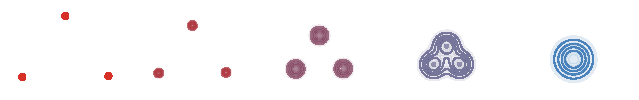
\includegraphics[width=.72\linewidth]{figures/generative-diffusion-2d-forward-backward/forward-density-linear.pdf} \\[.15em]
\small OU/variance-preserving bridge, $a_t=\cos(\pi t/2)$, $b_t=\sin(\pi t/2)$ \\[-.15em]
\index{bridge!OU}% strictindex
\index{bridge!variance-preserving}% strictindex
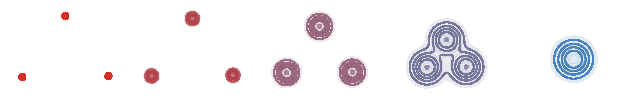
\includegraphics[width=.72\linewidth]{figures/generative-diffusion-2d-forward-backward/forward-density-ou.pdf}
\end{tabular}
\caption{Two-dimensional noising paths from three Dirac masses to a single Gaussian. The top row shows the linear interpolation $Z_t=(1-t)X+tY$, whose component centers move linearly toward the origin and whose covariance grows like $(t\sigma)^2\Id$. The bottom row uses the variance-preserving Ornstein--Uhlenbeck coefficients $a_\tau=e^{-\tau}$ and $b_\tau=\sqrt{1-e^{-2\tau}}$, reparametrized by $\tau=-\log\cos(\pi t/2)$ so that $a_t=\cos(\pi t/2)$ and $b_t=\sin(\pi t/2)$. It has the same endpoints but a different speed of contraction and noising.}
\index{Ornstein-Uhlenbeck process}% strictindex
\index{bridge!variance-preserving}% strictindex
\label{fig:generative-diffusion-2d-forward-backward}
\end{figure}

\paragraph{When is the induced map optimal?}

Integrating the learned velocity gives a deterministic map from $\alpha_0$ to $\alpha_1$, but this map is not automatically the Brenier optimal map. It is optimal only in special cases where the accumulated flow remains the gradient of a convex potential. The Gaussian product-coupling case already shows the precise obstruction: the interpolated covariances are simple, the velocity is affine, but the terminal map can contain a hidden rotational part. This phenomenon, and its extensions to rectified flows and mixtures, is analyzed in depth in~\cite{HertrichChambolleDelon2025RectifiedOT}.
\index{convex!potential}% strictindex
\index{product!coupling}% strictindex
\index{flow!rectified}% strictindex

\begin{prop}[Gaussian flow matching and optimality]\label{prop-gaussian-flow-matching-optimality}
\index{Gaussian!flow matching}% strictindex
	Let $\Sigma_0,\Sigma_1\succ0$ and let $X_0\sim\Gaussian(0,\Sigma_0)$ and $X_1\sim\Gaussian(0,\Sigma_1)$ be independent. Consider the linear flow-matching interpolation
\index{flow!matching}% strictindex
	\[
		Z_t=(1-t)X_0+tX_1,
		\qquad
		\alpha_t=\operatorname{Law}(Z_t)=\Gaussian(0,\Sigma_t),
	\]
	where
	\begin{equation}\label{eq-gaussian-product-fm-covariance}
		\Sigma_t=(1-t)^2\Sigma_0+t^2\Sigma_1.
	\end{equation}
	Then the exact flow-matching velocity is affine, $v_t(z)=A_tz$, with
\index{flow!matching}% strictindex
	\begin{equation}\label{eq-gaussian-product-fm-velocity}
		A_t=\bigl(t\Sigma_1-(1-t)\Sigma_0\bigr)\Sigma_t^{-1}.
	\end{equation}
	The induced flow map $T_t^{\rm FM}$ from $\alpha_0$ to $\alpha_t$ is
\index{flow!map}% strictindex
	\begin{equation}\label{eq-gaussian-product-fm-map}
		T_t^{\rm FM}
		=
		\Sigma_0^{1/2}
		\Bigl((1-t)^2\Id+t^2\Sigma_0^{-1/2}\Sigma_1\Sigma_0^{-1/2}\Bigr)^{1/2}
		\Sigma_0^{-1/2}.
	\end{equation}
	In particular,
	\begin{equation}\label{eq-gaussian-product-fm-terminal-map}
		T_1^{\rm FM}
		=
		\Sigma_0^{1/2}
		\bigl(\Sigma_0^{-1/2}\Sigma_1\Sigma_0^{-1/2}\bigr)^{1/2}
		\Sigma_0^{-1/2}.
	\end{equation}
	This terminal map coincides with the quadratic optimal transport map
\index{transport map}% strictindex
	\begin{equation}\label{eq-gaussian-brenier-map-comparison}
		T^{\rm OT}
		=
		\Sigma_0^{-1/2}
		\bigl(\Sigma_0^{1/2}\Sigma_1\Sigma_0^{1/2}\bigr)^{1/2}
		\Sigma_0^{-1/2}
	\end{equation}
	if and only if $\Sigma_0\Sigma_1=\Sigma_1\Sigma_0$.
\end{prop}

\begin{proof}
	The conditional-expectation formula gives
\index{conditional!expectation}% strictindex
	\[
		v_t(z)=\EE[X_1-X_0\mid Z_t=z].
	\]
	Since all variables are jointly Gaussian, this conditional expectation is linear and
\index{conditional!expectation}% strictindex
	\[
		v_t(z)
		=
		\operatorname{Cov}(X_1-X_0,Z_t)\operatorname{Cov}(Z_t)^{-1}z
		=
		\bigl(t\Sigma_1-(1-t)\Sigma_0\bigr)\Sigma_t^{-1}z,
	\]
	which proves~\eqref{eq-gaussian-product-fm-velocity}. To solve the characteristic equation, whiten the source by setting
	\[
		C=\Sigma_0^{-1/2}\Sigma_1\Sigma_0^{-1/2},
		\qquad
		\widetilde Z_t=\Sigma_0^{-1/2}Z_t.
	\]
	In these coordinates the source covariance is $\Id$ and
	\[
		\widetilde\Sigma_t=(1-t)^2\Id+t^2C.
	\]
	Because $\Id$ and $C$ commute, the affine flow map in whitened coordinates is simply $\widetilde T_t=\widetilde\Sigma_t^{1/2}$. Indeed,
\index{flow!map}% strictindex
	\[
		\frac{\d}{\d t}\widetilde\Sigma_t^{1/2}
		=
		\bigl(tC-(1-t)\Id\bigr)\widetilde\Sigma_t^{-1/2},
	\]
	which is exactly the equation $\dot{\widetilde T}_t=\widetilde A_t\widetilde T_t$ with $\widetilde T_0=\Id$. Returning to the original coordinates gives~\eqref{eq-gaussian-product-fm-map}, and $t=1$ gives~\eqref{eq-gaussian-product-fm-terminal-map}.

	Both $T_1^{\rm FM}$ and $T^{\rm OT}$ push $\Gaussian(0,\Sigma_0)$ to $\Gaussian(0,\Sigma_1)$. The Brenier map between nondegenerate Gaussians is the unique symmetric positive definite linear map with this property. Hence $T_1^{\rm FM}=T^{\rm OT}$ if and only if $T_1^{\rm FM}$ is symmetric positive definite. The map $T_1^{\rm FM}$ is similar to $C^{1/2}$, so if it is symmetric then it is automatically positive definite. It remains to characterize symmetry. Since $C^{1/2}$ is symmetric positive definite,
\index{Brenier!map}% strictindex
	\[
		(T_1^{\rm FM})^\top
		=
		\Sigma_0^{-1/2}C^{1/2}\Sigma_0^{1/2}.
	\]
	Thus symmetry of $T_1^{\rm FM}$ is equivalent to
	$\Sigma_0 C^{1/2}=C^{1/2}\Sigma_0$, hence to $\Sigma_0 C=C\Sigma_0$ by functional calculus. Multiplying this identity on the left and right by $\Sigma_0^{1/2}$ gives $\Sigma_0\Sigma_1=\Sigma_1\Sigma_0$. Conversely, if $\Sigma_0$ and $\Sigma_1$ commute, they are orthogonally co-diagonalizable, and both~\eqref{eq-gaussian-product-fm-terminal-map} and~\eqref{eq-gaussian-brenier-map-comparison} reduce in that basis to the diagonal map with entries $\sqrt{\lambda_{1,k}/\lambda_{0,k}}$. This proves the equivalence.
\index{Brenier!map}% strictindex
\end{proof}

The proposition gives a compact warning about a common overinterpretation of flow matching.

\begin{rem}[Changing the bridge speed does not restore optimality]
	The same terminal map~\eqref{eq-gaussian-product-fm-terminal-map} is obtained for any scalar schedule $Z_t=a_tX_0+b_tX_1$ with the same endpoints, because after whitening the covariance path remains $a_t^2\Id+b_t^2C$. Thus changing the speed of a scalar Gaussian bridge, for instance by using an OU schedule, cannot repair the non-optimality created by non-commuting covariances.

	Commuting covariances reduce the terminal map to independent one-dimensional scalings, whereas non-commuting covariances create a non-symmetric affine map, hence a transport with a rotational or shearing component. More generally, mixture-like paths can create the same obstruction even when every instantaneous velocity looks natural. This distinction is closely related to counterexamples showing that flow maps associated with Fokker--Planck or diffusion-type evolutions do not in general provide optimal transport maps~\cite{LavenantSantambrogio2022FlowMap}. In particular, starting from an isotropic Gaussian does not by itself guarantee optimality once the target distribution is non-Gaussian; additional structural assumptions on the path or on the coupling are needed.
\end{rem}
\index{affine map}% strictindex
\index{flow!map}% strictindex
\index{rotational component}% strictindex
\index{shearing component}% strictindex
\index{Lavenant criterion}% strictindex
\index{transport map}% strictindex
\index{Fokker-Planck equation}% strictindex
\index{flow!matching}% strictindex
\index{Gaussian!flow matching}% strictindex
\index{covariance!commuting}% strictindex
\index{flow!map}% strictindex

\paragraph{Variations on the interpolant.}

The geometry of the generated trajectories depends on the chosen interpolant, not only on the two endpoint laws. There is first a harmless ambiguity: a monotone reparametrization $Z_t=(1-\lambda(t))X+\lambda(t)Y$ of the linear bridge only changes the speed of the flow,
\[
	v_t(z)=\lambda'(t)\,v^{\rm lin}_{\lambda(t)}(z),
	\qquad
	v^{\rm lin}_{r}(z)=\EE[Y-X\mid (1-r)X+rY=z].
\]
It therefore leaves the spatial integral curves unchanged. Diffusion models use a genuinely different family of noising paths. If
\index{diffusion model}% strictindex
\[
	Z_t=a_tX+b_tY,\qquad Y\sim\Gaussian(0,\sigma^2\Id),
\]
then both the mixture centers and the component variances are changed. Writing $p_t$ for the density of $Z_t$ and $s_t=\nabla\log p_t$, Tweedie's formula gives, away from times where $a_t=0$,
\index{Tweedie identity}% strictindex
\[
	v_t(z)=a'_t\,\EE[X\mid Z_t=z]+b'_t\,\EE[Y\mid Z_t=z]
	=\frac{a'_t}{a_t}z+
	\left(\frac{a'_tb_t^2}{a_t}-b'_tb_t\right)\sigma^2s_t(z).
\]
For the linear bridge, $a_t=1-t$ and $b_t=t$, this recovers the formula above. For the variance-preserving Ornstein--Uhlenbeck noising used in diffusion models,
\index{Ornstein-Uhlenbeck process}% strictindex
\index{bridge!variance-preserving}% strictindex
\index{diffusion model}% strictindex
\[
	a_\tau=e^{-\tau},\qquad b_\tau=\sqrt{1-e^{-2\tau}},
\]
one obtains the forward probability-flow velocity $v_\tau(z)=-z-\sigma^2\nabla\log p_\tau(z)$. Sampling follows the reverse field $z+\sigma^2\nabla\log p_\tau(z)$ as $\tau$ decreases. This is the noising law used in the left panel of Figure~\ref{fig:generative-diffusion-versus-ot-2d}; the trajectories are more curved than for the linear bridge because the centers and variances evolve according to the OU/Fokker--Planck scaling rather than by affine interpolation. Numerically, the integration is stopped at a small positive time before the Dirac endpoint, where the score becomes singular.
\index{Fokker-Planck equation}% strictindex

The finite-time coefficients $a_t=\cos(\pi t/2)$ and $b_t=\sin(\pi t/2)$ are not a new spatial interpolant: they are exactly the OU coefficients after the time change $\tau=-\log\cos(\pi t/2)$. Figure~\ref{fig:generative-diffusion-schedule-comparison} therefore compares OU with a genuinely different scalar bridge,
\[
	a_t=(1-t)(1-2t),
	\qquad
	b_t=t,
\]
whose data coefficient changes sign before vanishing. This overshooting bridge is mainly a diagnostic example: it keeps the same endpoints, but its intermediate mixture reflects through the origin and produces visibly different reverse trajectories.
\index{bridge!overshooting}% strictindex

\begin{figure}[H]
\centering
\begin{tabular}{@{}cc@{}}
\small diffusion-like trajectories & \small OT displacement rays \\[-.15em]

\includegraphics[width=.39\linewidth]{figures/generative-diffusion-versus-ot-2d/diffusion-curves.pdf} &

\includegraphics[width=.39\linewidth]{figures/generative-diffusion-versus-ot-2d/ot-rays.pdf}
\end{tabular}
\caption{Diffusion-style sampling trajectories compared with OT rays in the three-Dirac setting of Figure~\ref{fig:generative-diffusion-2d-forward-backward}. Red particles are sampled from the centered Gaussian endpoint and transported toward the three blue atoms. The left panel integrates the reverse probability-flow ODE for the variance-preserving OU noising $a_\tau=e^{-\tau}$, $b_\tau=\sqrt{1-e^{-2\tau}}$, using the closed-form Gaussian-mixture score and stopping just before the singular Dirac endpoint. The right panel uses the straight displacement rays selected by a quadratic OT matching to the same atoms.}
\index{Gaussian mixture}% strictindex
\index{bridge!variance-preserving}% strictindex
\index{probability-flow ODE}% strictindex
\index{score function}% strictindex
\index{flow!probability ODE}% strictindex
\label{fig:generative-diffusion-versus-ot-2d}
\end{figure}

\begin{figure}[H]
\centering
\begin{tabular}{@{}ccc@{}}
\small linear bridge & \small OU VP bridge & \small overshooting bridge \\[-.15em]
\index{bridge!overshooting}% strictindex
\index{bridge!OU}% strictindex
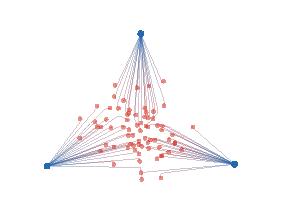
\includegraphics[width=.30\linewidth]{figures/generative-diffusion-versus-ot-2d/schedule-linear.pdf} &
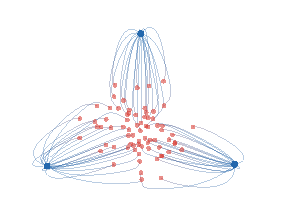
\includegraphics[width=.30\linewidth]{figures/generative-diffusion-versus-ot-2d/schedule-vp.pdf} &
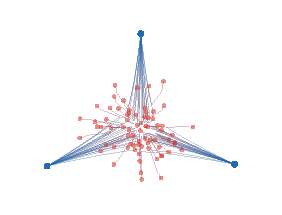
\includegraphics[width=.30\linewidth]{figures/generative-diffusion-versus-ot-2d/schedule-overshoot.pdf}
\end{tabular}
\caption{Effect of the interpolant on the exact reverse flow for the same three-Dirac target and the same Gaussian endpoint. The linear bridge $a_t=1-t$, $b_t=t$ produces almost radial curves. The variance-preserving OU bridge $a_\tau=e^{-\tau}$, $b_\tau=\sqrt{1-e^{-2\tau}}$ changes the relative speed of contraction and noising. The overshooting bridge $a_t=(1-t)(1-2t)$, $b_t=t$ is not a time reparameterization of either one and produces a more pronounced bending of the reverse trajectories.}
\index{reverse flow}% strictindex
\index{bridge!overshooting}% strictindex
\index{bridge!variance-preserving}% strictindex
\index{bridge!OU}% strictindex
\label{fig:generative-diffusion-schedule-comparison}
\end{figure}

%%%%%%%%%%%%%%%%%%%%%%%%%%%%%%%%%%%%%%%%%%%%%%%%%%%%%%%%%%%%%%%%%%%%%%%%%%%%%%%%%

\section{One-Step Generative Models}
\index{one-step!generative model}% strictindex

One-step generative models try to keep the geometric training principle of flows while removing the expensive multi-step integration at sampling time. The idea is to evolve the model distribution during training, but to store the final evolution in a single generator evaluation.
\index{generative model}% strictindex

\paragraph{Training a one-step flow.}
\index{one-step!flow}% strictindex

Let $\zeta$ be a simple latent distribution and let $\alpha_\theta=(G_\theta)_\sharp\zeta$ be the model distribution. Assume that the target data distribution is $\beta$. A Wasserstein-flow construction chooses a discrepancy
\[
	\mathcal E_\beta(\alpha),
\]
for instance a smoothed $\KL(\alpha|\beta)$, an MMD/IPM loss, or the debiased Sinkhorn divergence $\bar\MK_\c^\epsilon(\alpha,\beta)$ introduced in Section~\ref{sec-sinkhorn-div}. The associated formal descent is
\index{maximum mean discrepancy}% strictindex
\index{integral probability metric}% strictindex
\index{Sinkhorn!divergence}% strictindex
\begin{equation}\label{eq-one-step-wgf}
	\partial_t\mu_t+\diverg(\mu_t w_t)=0,
	\qquad
	w_t(x)=-\nabla\delta_\alpha \mathcal E_\beta(\mu_t)(x).
\end{equation}
Instead of integrating~\eqref{eq-one-step-wgf} at inference time, one fits a parametric residual field $U_\eta$ along the current model distribution:
\begin{equation}\label{eq-one-step-l2-fit}
	\min_\eta \int_0^1\!\int
		\norm{U_\eta(t,x)-w_t(x)}^2
		\,\d\mu_t(x)\,\d t.
\end{equation}
In a particle or generator implementation, the learned residual is then used to update the current generator by
\[
	\alpha_{\theta}^{+}
	=
	(\Id+\tau U_\eta)_\sharp \alpha_\theta,
	\qquad\text{or equivalently}\qquad
	G_\theta^{+}(z)=G_\theta(z)+\tau U_\eta(G_\theta(z)).
\]

\begin{alg}[One-step Wasserstein-flow generator update]\label{alg:one-step-wgf-generator-update}
\index{one-step!generative model}% strictindex
\textbf{Input:} Generator $G_{\theta_k}$, latent law $\zeta$, data law $\beta$, numerical descent-field oracle $W_\beta$, step size $\tau$, batch size $B$.

\textbf{Output:} Updated generator $G_{\theta_{k+1}}$.

\textbf{Draw} $z_b\sim\zeta$ for $b=1,\ldots,B$.

\textbf{Set} $x_b=G_{\theta_k}(z_b)$.

\textbf{Set} \(w_k(x)=W_\beta[\alpha_{\theta_k}](x)\), where \(W_\beta[\alpha]=-\nabla\delta_\alpha\mathcal E_\beta(\alpha)\).

\textbf{Set} $\eta_k$ by minimizing the empirical least-squares loss:
\(\frac1B\sum_{b=1}^B \norm{U_{\eta}(x_b)-w_k(x_b)}^2.\)

\textbf{Update by composition:}
\(G_{\theta_{k+1}}(z) = G_{\theta_k}(z)+\tau U_{\eta_k}(G_{\theta_k}(z)).\)

\textbf{Return} $G_{\theta_{k+1}}$.
\end{alg}

After many training updates, the accumulated generator is evaluated once at test time. This is the organizing principle behind recent one-step methods based on Wasserstein gradient flows: W-Flow uses such a construction with the Sinkhorn divergence as a tractable global discrepancy~\cite{Han2026WFlow}, while drifting methods evolve the generated distribution during training through a fitted vector field and also admit one-step inference~\cite{Deng2026Drifting}. The gradient-flow interpretation of drifting models, and its relation to KL, MMD, sliced-Wasserstein and Sinkhorn-type discrepancies, is analyzed in~\cite{Gretton2026DriftingWGF,He2026SinkhornDrifting}. These ideas are also connected to the Sinkhorn-type normalization dynamics used to model attention in Sinkformers~\cite{Sander2022Sinkformers}.
\index{Wasserstein!gradient}% strictindex
\index{gradient!flow}% strictindex
\index{Wasserstein!gradient flow}% strictindex
\index{Sinkhorn!divergence}% strictindex
\index{drifting!model}% strictindex

\paragraph{Self-corrected drifting fields.}
\index{drifting!field}% strictindex

Drifting methods need not start from an exact Wasserstein gradient. They often prescribe an attraction-minus-repulsion field and then regress this field in $L^2(\mu_t)$. A simple continuous version uses a positive kernel $K_\epsilon(x,y)$ and defines, for any measure $\nu$,
\index{Wasserstein!gradient}% strictindex
\index{kernel!positive}% strictindex
\begin{equation}\label{eq-normalized-kernel-drift}
	B_\epsilon[\nu](x)
	\eqdef
	\frac{\int (y-x)K_\epsilon(x,y)\,\d\nu(y)}
	     {\int K_\epsilon(x,y)\,\d\nu(y)}.
\end{equation}
For the Gaussian kernel
\index{kernel!Gaussian}% strictindex
$K_\epsilon(x,y)=\exp(-\norm{x-y}^2/(2\epsilon))$, this normalized field is a score of a smoothed density:
\index{score function}% strictindex
\begin{equation}\label{eq-normalized-kernel-score}
	B_\epsilon[\nu](x)
	=
	\epsilon\nabla\log\!\left(\int K_\epsilon(x,y)\,\d\nu(y)\right).
\end{equation}
The drifting velocity is then
\begin{equation}\label{eq-cross-minus-self-drift}
	u_t(x)=B_\epsilon[\beta](x)-B_\epsilon[\mu_t](x)
	=
	\epsilon\nabla\log
	\frac{\int K_\epsilon(x,y)\,\d\beta(y)}
	     {\int K_\epsilon(x,y)\,\d\mu_t(y)}.
\end{equation}
The first term pulls samples toward data, while the second term corrects self-attraction and prevents all particles from collapsing onto the same high-density region. Sinkhorn drifting replaces these one-sided kernel normalizations by two-sided entropic OT couplings, so that the cross and self terms are normalized by Sinkhorn scaling rather than by a single denominator~\cite{He2026SinkhornDrifting}.
\index{Sinkhorn!scaling}% strictindex
\index{kernel!norm}% strictindex
\index{entropic!OT}% strictindex

\begin{alg}[Self-corrected drifting particle update]\label{alg:self-corrected-drifting-particles}
\index{drifting!model}% strictindex
\textbf{Input:} Particles $x_i^k$ for $\mu_k$, data samples $(y_b)_{b=1}^B$ from $\beta$, kernel scale $\epsilon$, step $h$.

\textbf{Output:} Updated particles $x_i^{k+1}$.

\textbf{For} each particle $i$ \textbf{do}:
\begin{algblock}

\textbf{Set} \(Z_{\beta,i}=\sum_{b=1}^B K_\epsilon(x_i^k,y_b)\) and \(b_i^k=Z_{\beta,i}^{-1}\sum_{b=1}^B (y_b-x_i^k)K_\epsilon(x_i^k,y_b)\).

\textbf{Set} \(Z_{\mu,i}=\sum_{j=1}^n K_\epsilon(x_i^k,x_j^k)\) and \(m_i^k=Z_{\mu,i}^{-1}\sum_{j=1}^n (x_j^k-x_i^k)K_\epsilon(x_i^k,x_j^k)\).

\textbf{Set}
\(u_i^k=b_i^k-m_i^k.\)

\textbf{Update}
\(x_i^{k+1}=x_i^k+h\,u_i^k.\)
\end{algblock}
\textbf{Return} $(x_i^{k+1})_i$.
\end{alg}

\begin{figure}[ht]
\centering
\begin{tabular}{@{}cc@{}}

\includegraphics[width=.38\linewidth]{figures/generative-drifting-model-trajectories/unnormalized-trajectories.pdf} &
\index{drifting!model}% strictindex
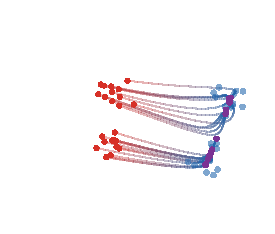
\includegraphics[width=.38\linewidth]{figures/generative-drifting-model-trajectories/normalized-trajectories.pdf}
\\[-.1em]
\small raw kernel drift & \small self-corrected drift
\index{self-corrected field}% strictindex
\end{tabular}
\caption{Drifting trajectories for a small particle generator. The raw Laplacian-kernel drift has weak long-range attraction and can leave particles away from the data modes. The self-corrected field uses the difference $B_\epsilon[\beta]-B_\epsilon[\mu_t]$, so a longer integration brings particles to the blue modes while repelling them from their own current concentration.}
\label{fig:generative-drifting-model-trajectories}
\end{figure}

\begin{prop}[Drifting as a time-dependent Wasserstein gradient]\label{prop-drifting-semi-relaxed-gradient}
\index{drifting!model}% strictindex
\index{Wasserstein!gradient}% strictindex
	Let $\mu_t$ be a smooth curve of positive densities and let $u_t=\nabla\phi_t$ be a smooth time-dependent gradient field. Define the semi-relaxed functional
	\begin{equation}\label{eq-semi-relaxed-drift-functional}
		\mathcal R_t(\alpha|\mu_t)
		\eqdef
		-\int \phi_t(x)\,\d\alpha(x)
		+\int \phi_t(x)\,\d\mu_t(x).
	\end{equation}
	Here $\mu_t$ and $\phi_t$ are frozen when taking the first variation with respect to the first argument $\alpha$. Then the continuity equation
\index{first variation}% strictindex
\index{continuity equation}% strictindex
	\[
		\partial_t\mu_t+\diverg(\mu_t u_t)=0
	\]
	is the formal Wasserstein gradient descent of the time-dependent functional $\alpha\mapsto\mathcal R_t(\alpha|\mu_t)$.
\index{Wasserstein!gradient}% strictindex
\end{prop}

\begin{proof}
	Since $\mu_t$ and $\phi_t$ are fixed in the variation with respect to $\alpha$, the first variation is
\index{first variation}% strictindex
	\[
		\delta_\alpha \mathcal R_t(\alpha|\mu_t)(x)=-\phi_t(x).
	\]
	By Proposition~\ref{prop-formal-wass-gradient},
	\[
		\Wgrad \mathcal R_t(\alpha|\mu_t)
		=
		\nabla\delta_\alpha \mathcal R_t(\alpha|\mu_t)
		=
		-\nabla\phi_t
		=
		-u_t.
	\]
	The Wasserstein gradient-descent velocity is the negative of this gradient, namely $u_t$. Substituting this velocity in the continuity equation gives the claimed flow.
\index{Wasserstein!gradient}% strictindex
\index{continuity equation}% strictindex
\end{proof}

\begin{example}[Kernel drifting as a semi-relaxed divergence]
\index{Gaussian!kernel drifting}% strictindex
\index{kernel!drifting}% strictindex
\index{semi-relaxed!divergence}% strictindex
	For the Gaussian-kernel drift~\eqref{eq-cross-minus-self-drift}, set
	\[
		\phi_t(x)=
		\epsilon\log
		\frac{\int K_\epsilon(x,y)\,\d\beta(y)}
		     {\int K_\epsilon(x,y)\,\d\mu_t(y)}.
	\]
	Then $u_t=\nabla\phi_t$, so Proposition~\ref{prop-drifting-semi-relaxed-gradient} shows that kernel drifting is the Wasserstein gradient descent of
\index{Wasserstein!gradient}% strictindex
\index{kernel!drifting}% strictindex
	\[
		\mathcal R_t^{\mathrm{drift}}(\alpha|\mu_t)
		=
		\epsilon
		\int
		\log
		\frac{\int K_\epsilon(x,y)\,\d\mu_t(y)}
		     {\int K_\epsilon(x,y)\,\d\beta(y)}
		\,\d\alpha(x)
		+\mathrm{constant}.
	\]
	It is ``semi-relaxed'' because the current model $\mu_t$ is used to build the potential, but it is not varied inside the denominator when computing the first variation in $\alpha$.
\index{first variation}% strictindex
\end{example}

\begin{rem}[General fields and projection onto gradients]
\index{gradient!projection}% strictindex
	A general regressed field $b_t$ is not necessarily a Wasserstein gradient, since Wasserstein tangent vectors are represented by gradient fields modulo $L^2(\mu_t)$-null directions. The gradient component is obtained by the weighted projection
\index{Wasserstein!gradient}% strictindex
	\[
		\nabla\phi_t
		=
		\uargmin{\nabla\phi}
		\int \norm{\nabla\phi(x)-b_t(x)}^2\,\d\mu_t(x).
	\]
	One may first normalize $b_t$ pointwise, for instance by $b_t/(\norm{b_t}+\eta)$, or globally by $\norm{b_t}_{L^2(\mu_t)}$, before this projection. Proposition~\ref{prop-drifting-semi-relaxed-gradient} then applies to the projected field. Non-gradient components can still be useful in a parametric model, but they are not descent directions of a scalar functional for the $\Wass_2$ Riemannian metric.
\end{rem}

\section{Evolution in Depth of Transformers}
\index{transformer}% strictindex
\index{depth evolution}% strictindex

Deep residual architectures can be read as time discretizations of ODEs or PDEs. For transformers, the transported objects are token measures and the velocity is induced by attention.
\index{token measure}% strictindex

Transformers were introduced as sequence-to-sequence architectures driven by self-attention~\cite{Vaswani2017Attention} and have since become a central architecture for language and vision models~\cite{Brown2020LanguageModels,Dosovitskiy2021Image}. Their distinctive feature is that each token is updated by a data-dependent average of all other tokens. This makes an attention layer permutation-equivariant before positional encoding, context dependent after conditioning on the input sequence, and naturally compatible with a measure viewpoint in which a prompt is regarded as an empirical distribution of tokens.
\index{transformer}% strictindex
\index{empirical!distribution}% strictindex
\index{attention!self-attention}% strictindex

The mathematical limit used below concerns depth rather than model scale: one lets the number of residual attention layers grow while each layer makes a small update, as in continuous-depth neural networks~\cite{Chen2018NeuralODE}. For attention, the resulting velocity is nonlinear in the current token law because it is normalized by the whole context. This measure-theoretic view appears in the analysis of attention as a Lipschitz or interacting-particle operator~\cite{Vuckovic2020MathematicalAttention,Geshkovski2023MathematicalPerspective}, in the Sinkhorn-normalized dynamics of Sinkformers~\cite{Sander2022Sinkformers}, and in recent well-posedness and mean-field-limit results for several attention mechanisms~\cite{Castin2025DynamicsTransformers}. It also separates the infinite-depth limit studied here from the token-limit question, where one controls how a finite empirical context approximates its limiting attention operator~\cite{Bohbot2025TokenSampleComplexity}.
\index{empirical context}% strictindex
\index{attention!operator}% strictindex
\index{infinite-depth limit}% strictindex
\index{token limit}% strictindex
\index{transformer}% strictindex
\index{mean-field!limit}% strictindex
\index{attention!mechanism}% strictindex
\index{continuous!depth}% strictindex

We now consider very deep transformers, focusing on a single-head attention mechanism for simplicity while ignoring MLP layers, layer normalization, causality, and masking. This stripped-down framework is best suited to modeling encoders and vision transformers; the references above indicate which parts of this simplified picture extend to richer attention mechanisms.
\index{attention!single-head}% strictindex
\index{layer normalization}% strictindex
\index{causality}% strictindex
\index{masking}% strictindex
\index{transformer}% strictindex

\paragraph{Attention as a context-dependent velocity.}
\index{attention}% strictindex
\index{velocity field}% strictindex

After tokenization, embedding, and positional encoding, each input (from a set of tokens) is represented as a point cloud $(x_i)_{i=1}^n$ of $n$ points in the space of vectorized tokens. An attention layer with skip connection and rescaling by $1/T$ (where $T$ is the depth) defines a transformation of the tokens:
\begin{equation*}
    x_i \mapsto x_i + \frac{1}{T} \sum_j \frac{e^{\langle Q x_i, K x_j \rangle} V x_j}{\sum_{\ell} e^{\langle Q x_i, K x_\ell \rangle}},
\end{equation*}
where $\theta = (K, Q, V)$ are the parameters of the attention layer, represented by three matrices.

\paragraph{Token measure evolution.}
\index{token measure}% strictindex

To handle an arbitrary number of tokens, we define $\alpha = \frac{1}{n} \sum_i \delta_{x_i}$ as the empirical measure of tokens and rewrite the transformer mapping as:
\index{empirical!measure}% strictindex
\index{transformer}% strictindex
\begin{equation*}
    x_i \mapsto x_i + \frac{1}{T} \Gamma_\theta[\alpha](x_i),
\end{equation*}
where
\begin{equation*}
    \Gamma_\theta[\alpha](x) :=
    \frac{\int e^{\langle Q x, K y \rangle} V y \, \d \alpha(y)}
    {\int e^{\langle Q x, K z \rangle} \, \d \alpha(z)}.
\end{equation*}
At the level of the token distribution, the layer pushes $\alpha$ forward by the ``in-context'' mapping $\Gamma_{\theta_t}[\alpha]$, which depends on the context $\alpha$, the tokens, and the depth-dependent parameters $\theta_t$. Denoting $t \in [0, 1]$ as the depth and $\tau = 1/T$ as the step size, this gives:
\begin{equation*}
    \alpha_{t+\tau} = (\Id + \tau \Gamma_{\theta_t}[\alpha_t])_\sharp \alpha_t.
\end{equation*}
As $\tau \to 0$, this converges formally to the conservation equation
\begin{equation*}
    \partial_t \alpha_t + \diverg(\alpha_t \Gamma_{\theta_t}[\alpha_t]) = 0.
\end{equation*}

\begin{alg}[Residual attention depth evolution]\label{alg:residual-attention-depth-evolution}
\index{attention!self-attention}% strictindex
\index{transformer}% strictindex
\textbf{Input:} Tokens $(x_i^0)_{i=1}^n$, depth $T$, layer parameters $(Q_k,K_k,V_k)$.

\textbf{Output:} Final token measure $\alpha_T$.

\textbf{Initialize:}
\(\alpha_0=\frac1n\sum_{i=1}^n\delta_{x_i^0}, \qquad \tau=1/T.\)

\textbf{For} $k=0,\ldots,T-1$ \textbf{do}:
\begin{algblock}

\textbf{For} $i=1,\ldots,n$ \textbf{do}
\begin{algblock}
\(\Gamma_{\theta_k}[\alpha_k](x_i^k) = \frac{\sum_j \exp(\dotp{Q_kx_i^k}{K_kx_j^k})\,V_kx_j^k} {\sum_j \exp(\dotp{Q_kx_i^k}{K_kx_j^k})}.\)

\(x_i^{k+1}=x_i^k+\tau\,\Gamma_{\theta_k}[\alpha_k](x_i^k).\)
\end{algblock}
\textbf{Set}
\(\alpha_{k+1}=(\Id+\tau\Gamma_{\theta_k}[\alpha_k])_\sharp\alpha_k.\)
\end{algblock}
\textbf{Return} $\alpha_T$.
\end{alg}

\paragraph{Gradient structure and limitations.}
\index{gradient!structure}% strictindex

When the token space has dimension $d$ and the query/key space has dimension $r$, take $Q,K\in\RR^{r\times d}$ and $V\in\RR^{d\times d}$. If $V=Q^\top K$, the field $\Gamma_\theta[\alpha]$ is a gradient vector field in the token variable. Indeed, define the log-partition potential
\[
	\Phi_\alpha(x)
	=
	\int \exp(\dotp{Qx}{Ky})\d\alpha(y),
	\qquad
	U_\alpha(x)=\log\Phi_\alpha(x).
\]
Then
\[
	\nabla_x U_\alpha(x)
	=
	\frac{\int Q^\top K y\,\exp(\dotp{Qx}{Ky})\d\alpha(y)}
	     {\int \exp(\dotp{Qx}{Kz})\d\alpha(z)}
	=
	\Gamma_\theta[\alpha](x).
\]
This is an instantaneous gradient in $x$. It is not, however, the gradient of the first variation of a fixed functional of $\alpha$, because the potential $U_\alpha$ itself depends on the current measure through the same attention normalization. Thus the PDE is generally a transportation dynamics, not a Wasserstein gradient flow. Special variants recover additional structure: Sinkhorn attention can be interpreted through doubly stochastic normalization and Wasserstein-type gradient flows~\cite{Sander2022Sinkformers,Castin2025DynamicsTransformers}, while layer normalization leads naturally to dynamics on the sphere and to modified metrics. The key open difficulty for the present viewpoint is training: after the architecture has been rewritten as a controlled transport equation, learning corresponds to optimizing the time-dependent parameters $(\theta_t)_t$ rather than merely analyzing the forward PDE for fixed parameters.
\index{doubly stochastic normalization}% strictindex
\index{transport equation}% strictindex
\index{controlled transport}% strictindex
\index{first variation}% strictindex
\index{layer normalization}% strictindex
\index{Wasserstein!gradient}% strictindex
\index{gradient!flow}% strictindex
\index{transformer}% strictindex
\index{Wasserstein!gradient flow}% strictindex

\section{Flows over the Gaussian Manifold}
\index{Gaussian!manifold}% strictindex

Gaussian measures provide a useful testing ground for the preceding dynamics. They are not invariant under a general Wasserstein gradient flow: a nonlinear velocity usually creates non-Gaussian densities immediately. The useful substitute is to either identify affine velocities, which exactly preserve Gaussianity, or to project the dynamics onto the Gaussian manifold. In both cases the measure PDE reduces to matrix ODEs for the mean and covariance. This viewpoint is emphasized in the survey~\cite{Peyre2026OptimalDiffusionTransports} and is useful for comparing diffusion paths, Wasserstein gradient flows, drifting fields and transformer-type dynamics.
\index{affine!closure}% strictindex
\index{drifting!field}% strictindex
\index{Wasserstein!gradient}% strictindex
\index{gradient!flow}% strictindex
\index{transformer}% strictindex
\index{Wasserstein!gradient flow}% strictindex
\index{Gaussian!manifold}% strictindex
\index{Gaussian!measure}% strictindex

For constrained gradient flows on this family, the covariance equation is the finite-dimensional Bures--Wasserstein gradient flow on positive definite matrices. Thus Gaussian closure is not just a computational shortcut: it is the restriction of Wasserstein geometry to the Gaussian submanifold, where affine gradient fields encode tangent vectors.
\index{Gaussian!submanifold}% strictindex
\index{affine!gradient}% strictindex
\index{Bures-Wasserstein geometry}% strictindex
\index{Wasserstein!gradient}% strictindex
\index{Gaussian!closure}% strictindex
\index{gradient!flow}% strictindex

\begin{figure}[ht]
\centering
\begin{tabular}{@{}ccc@{}}
\small $W_2$ geodesic & \small Sinkhorn closure & \small drifting closure \\[-.15em]
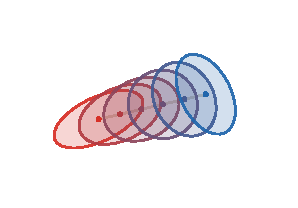
\includegraphics[width=.30\linewidth]{figures/gradflow-gaussian-closure/ot-ellipses.pdf} &
\index{Gaussian!closure}% strictindex
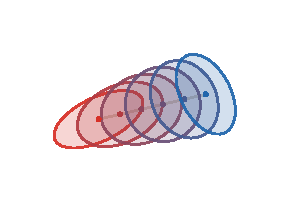
\includegraphics[width=.30\linewidth]{figures/gradflow-gaussian-closure/sinkhorn-ellipses.pdf} &
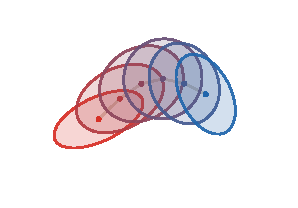
\includegraphics[width=.30\linewidth]{figures/gradflow-gaussian-closure/drifting-ellipses.pdf}
\end{tabular}
\caption{Gaussian closures of transport dynamics between two overlapping anisotropic Gaussians. The left panel is the exact $W_2$ Gaussian geodesic. The middle panel shows a regularized Sinkhorn-style closure, where the same mean path is accompanied by inflated intermediate covariances. The right panel shows a drifting-style closure with a curved mean path and moment-matched covariance ellipses. These finite-dimensional pictures keep only means and covariances, and therefore discard higher-order shape information that would be created by a genuinely nonlinear velocity field.}
\index{moment matching}% strictindex
\index{Gaussian!closure}% strictindex
\index{velocity field}% strictindex
\label{fig:gradflow-gaussian-closure}
\end{figure}

\paragraph{Gaussianity preservation.}
\index{Gaussian!preservation}% strictindex

The first question is invariance: one wants a simple criterion ensuring that the continuity equation does not leave the finite-dimensional Gaussian family.
\index{continuity equation}% strictindex

\begin{prop}[Affine velocities preserve Gaussianity]\label{prop-gaussian-affine-closure}
\index{Gaussian!preservation}% strictindex
\index{affine!closure}% strictindex
	Let $\alpha_t=\Gaussian(\mean_t,\cov_t)$, with $\cov_t$ positive definite, solve the continuity equation with an affine velocity
	\[
		v_t(x)=b_t+A_t(x-\mean_t).
	\]
	Then $\alpha_t$ remains Gaussian and its moments solve
	\[
		\dot \mean_t=b_t,
		\qquad
		\dot\cov_t=A_t\cov_t+\cov_t A_t^\top .
	\]
	Conversely, any smooth Gaussian curve with positive definite covariance can be generated by such an affine velocity. If one wants the velocity to be a Wasserstein tangent gradient, one chooses the unique symmetric solution of the Lyapunov equation
\index{affine!closure}% strictindex
\index{Lyapunov equation}% strictindex
	\[
		A_t\cov_t+\cov_t A_t=\dot\cov_t.
	\]
\end{prop}

\begin{proof}
	Let $X_t$ follow the characteristic ODE $\dot X_t=b_t+A_t(X_t-\mean_t)$. This linear ODE maps Gaussian random variables to Gaussian random variables. Taking expectation gives $\dot\mean_t=b_t$. Writing $\tilde X_t=X_t-\mean_t$, one has $\dot{\tilde X}_t=A_t\tilde X_t$, hence
\index{random variable}% strictindex
	\[
		\dot\cov_t
		=
		\frac{\d}{\d t}\EE(\tilde X_t\tilde X_t^\top)
		=
		A_t\cov_t+\cov_t A_t^\top .
	\]
	For the converse, set $b_t=\dot\mean_t$ and choose any matrix $A_t$ satisfying the covariance equation. Since $\cov_t$ is positive definite, the Lyapunov map $A\mapsto A\cov_t+\cov_t A$ is invertible on symmetric matrices, which gives the unique symmetric choice when a gradient velocity is required. In that case $v_t$ is the gradient of the quadratic potential $x\mapsto \dotp{b_t}{x}+\dotp{A_t(x-\mean_t)}{x-\mean_t}/2$.
\index{quadratic!potential}% strictindex
\index{gradient!velocity}% strictindex
\end{proof}

\paragraph{Constrained evolution on the Gaussian manifold.}
\index{Gaussian!manifold}% strictindex

For non-affine velocities, the finite-dimensional substitute is to project the Wasserstein dynamics onto the Gaussian manifold.
\index{affine!closure}% strictindex
\index{Gaussian!manifold}% strictindex

Let
\[
	\mathcal G=\{\Gaussian(\mean,\cov):\mean\in\RR^d,\ \cov\succ0\}
\]
be the Gaussian submanifold of $\Pp_2(\RR^d)$. The Wasserstein gradient of a functional constrained to a smooth submanifold $\mathcal M\subset\Pp_2$ is defined as the Riesz representative of the differential restricted to tangent velocities of $\mathcal M$. Equivalently, it is the small-step limit of the constrained JKO scheme
\index{Gaussian!submanifold}% strictindex
\index{Wasserstein!gradient}% strictindex
\index{JKO scheme}% strictindex
\[
	\alpha^{k+1}\in
	\uargmin{\alpha\in\mathcal M}
	\frac{1}{2\tau}\Wass_2^2(\alpha,\alpha^k)+f(\alpha).
\]
For $\mathcal M=\mathcal G$, tangent velocities are affine gradient fields $v(x)=b+A(x-\mean)$ with $A=A^\top$. The constrained gradient is therefore the $L^2(\Gaussian(\mean,\cov))$ projection of the ambient Wasserstein gradient onto this finite-dimensional affine space, whenever the ambient gradient exists.
\index{affine!gradient}% strictindex
\index{Wasserstein!gradient}% strictindex

\begin{prop}[Gaussian-constrained Wasserstein gradients]\label{prop-gaussian-gradient-bullet-list}
\index{Wasserstein!gradient}% strictindex
	Let $f$ be a smooth functional and assume that its restriction to nondegenerate Gaussian measures can be written as
\index{Gaussian!measure}% strictindex
	\[
		f(\Gaussian(\mean,\cov))=F(\mean,\cov).
	\]
	Then the Wasserstein gradient constrained to the Gaussian family is the affine vector field
\index{Wasserstein!gradient}% strictindex
	\[
		v_F(x)
		=
		\nabla_\mean F(\mean,\cov)
		+
		2\nabla_\cov F(\mean,\cov)(x-\mean),
	\]
	where $\nabla_\cov F$ denotes the symmetric matrix derivative. Equivalently, $v_F$ is the $L^2(\Gaussian(\mean,\cov))$ projection of the ambient Wasserstein gradient onto affine gradient fields, whenever the ambient gradient exists. Hence the gradient descent flow constrained to Gaussian measures satisfies
\index{affine!gradient}% strictindex
\index{Wasserstein!gradient}% strictindex
\index{Gaussian!measure}% strictindex
	\begin{equation}\label{eq-gaussian-wgf-closure}
		\dot\mean_t=-\nabla_\mean F(\mean_t,\cov_t),
		\qquad
		\dot\cov_t=-2\bigl(\cov_t\nabla_\cov F(\mean_t,\cov_t)+\nabla_\cov F(\mean_t,\cov_t)\cov_t\bigr),
	\end{equation}
	and the descent velocity is affine.
\end{prop}

\begin{proof}
	Test the functional along a Gaussian tangent vector, represented by an affine gradient field
\index{affine!gradient}% strictindex
	\[
		v(x)=b+A(x-\mean)
	\]
	with $A$ symmetric. The induced first-order variations are $\dot\mean=b$ and $\dot\cov=A\cov+\cov A$. Therefore
	\[
		\d F(\mean,\cov)[b,A\cov+\cov A]
		=
		\dotp{\nabla_\mean F}{b}
		+
		\mathrm{tr}\!\left(\nabla_\cov F(A\cov+\cov A)\right).
	\]
	Since $A$, $\cov$ and $\nabla_\cov F$ are symmetric, the second term equals
	\[
		2\,\mathrm{tr}(\nabla_\cov F\,A\cov)
		=
		\int \dotp{2\nabla_\cov F(x-\mean)}{A(x-\mean)}\d\Gaussian(\mean,\cov)(x).
	\]
	Together with the mean term, this gives
	\[
		\d F(\mean,\cov)[\dot\mean,\dot\cov]
		=
		\int \dotp{v_F(x)}{v(x)}\d\Gaussian(\mean,\cov)(x)
	\]
	for all affine gradient fields $v$. This identifies the constrained Wasserstein gradient in the induced $L^2(\alpha)$ metric, or equivalently the projection of the ambient gradient when it exists. Substituting the descent velocity $-v_F$ in Proposition~\ref{prop-gaussian-affine-closure} gives~\eqref{eq-gaussian-wgf-closure}.
\index{Wasserstein!gradient}% strictindex
\index{affine!closure}% strictindex
\end{proof}

This proposition should be read as the organizing rule for Gaussian closures: once the scalar energy has been reduced to a function of $(\mean,\cov)$, its constrained Wasserstein gradient is automatically affine and the covariance follows the Bures-type ODE~\eqref{eq-gaussian-wgf-closure}. When the first variation of $f$ is quadratic, this constrained gradient coincides with the full Wasserstein gradient.
\index{first variation}% strictindex
\index{Gaussian!closure}% strictindex

\paragraph{Gaussian-preserving gradient flows.}
\index{Gaussian!preservation}% strictindex
\index{gradient!flow}% strictindex

The next examples show that many familiar energies already have affine Wasserstein gradients on Gaussian inputs, so their full flow remains inside the Gaussian family.
\index{Wasserstein!gradient}% strictindex

\begin{example}[Gaussian energies and affine gradients]\label{ex-gaussian-affine-gradients}
\index{Gaussian!energy}% strictindex
\index{affine!gradient}% strictindex
	Proposition~\ref{prop-gaussian-gradient-bullet-list} turns many standard energies into explicit affine fields:
	\begin{itemize}
		\item \emph{Quadratic potential energy.} If
\index{quadratic!potential}% strictindex
		\[
			f(\alpha)=\int \Bigl(\frac12 x^\top Hx+\dotp{\ell}{x}\Bigr)\d\alpha(x),
			\qquad H=H^\top,
		\]
		then
		\[
			\Wgrad f(\alpha)(x)=Hx+\ell=(H\mean+\ell)+H(x-\mean).
		\]
		This is the Gaussian form of transport under a quadratic confinement.

		\item \emph{Quadratic interaction energy.} If
\index{energy!interaction}% strictindex
		\[
			f(\alpha)=\frac14\iint (x-y)^\top G(x-y)\d\alpha(x)\d\alpha(y),
			\qquad G=G^\top,
		\]
		then $F(\mean,\cov)=\frac12\mathrm{tr}(G\cov)$ and
		\[
			\Wgrad f(\alpha)(x)=G(x-\mean).
		\]
		The mean is unchanged and the covariance contracts or expands according to the signs of $G$.

		\item \emph{Relative entropy to a Gaussian.} For $\bar\alpha=\Gaussian(\bar\mean,\bar\cov)$,
\index{entropy!relative}% strictindex
		\[
			f(\alpha)=\KL(\alpha|\bar\alpha)
		\]
		has
		\[
			\Wgrad f(\alpha)(x)
			=
			\bar\cov^{-1}(\mean-\bar\mean)
			+
			(\bar\cov^{-1}-\cov^{-1})(x-\mean).
		\]
		The descent equations are the Ornstein--Uhlenbeck moment equations
\index{Ornstein-Uhlenbeck process}% strictindex
		\[
			\dot\mean_t=-\bar\cov^{-1}(\mean_t-\bar\mean),
			\qquad
			\dot\cov_t=2\Id-\bar\cov^{-1}\cov_t-\cov_t\bar\cov^{-1}.
		\]

		\item \emph{Squared Wasserstein distance to a Gaussian.} For
\index{Wasserstein!distance}% strictindex
		\[
			f(\alpha)=\frac12\Wass_2^2(\alpha,\bar\alpha),
			\qquad
			\bar\alpha=\Gaussian(\bar\mean,\bar\cov),
		\]
		the Gaussian Brenier map $T_{\alpha\to\bar\alpha}$ is affine,
\index{Brenier!map}% strictindex
		\[
			T_{\alpha\to\bar\alpha}(x)=\bar\mean+M(x-\mean),
			\qquad
			M=\cov^{-1/2}(\cov^{1/2}\bar\cov\cov^{1/2})^{1/2}\cov^{-1/2}.
		\]
		Hence
		\[
			\Wgrad f(\alpha)(x)=x-T_{\alpha\to\bar\alpha}(x)
			=
			(\mean-\bar\mean)+(\Id-M)(x-\mean),
		\]
		and descent moves each Gaussian infinitesimally along the Bures--Wasserstein geodesic toward $\bar\alpha$.
\index{Wasserstein!geodesic}% strictindex
\index{Bures-Wasserstein geometry}% strictindex

		\item \emph{Gaussian-only losses.} Sliced $\SW_2^2$ losses to a Gaussian, Gaussian Sinkhorn divergences, and any smooth closed formula depending only on $(\mean,\cov)$ fit the same constrained-gradient template:
\index{Gaussian!Sinkhorn}% strictindex
\index{Gaussian!Sinkhorn divergence}% strictindex
\index{Sinkhorn!divergence}% strictindex
			\[
				v_F(x)=\nabla_\mean F+2\nabla_\cov F(x-\mean).
			\]
		For Gaussian Sinkhorn divergences this finite-dimensional flow is studied in~\cite{HardionLacombe2026GaussianSinkhornFlow}.
\index{Gaussian!Sinkhorn divergence}% strictindex
\index{Sinkhorn!divergence}% strictindex
	\end{itemize}

	Not every PDE preserves Gaussianity exactly. For instance, Wasserstein flows of relative Fisher information, related to quantum-drift or higher-order diffusion equations, typically require a Gaussian projection to close on $(\mean,\cov)$. Such projected closures are still useful: they expose the finite-dimensional dynamics predicted by a variational model and make it easy to compare variational flows with non-variational affine dynamics such as drifting fields or the Gaussian transformer closure below.
\index{drifting!field}% strictindex
\index{transformer}% strictindex
\index{Gaussian!projection}% strictindex
\index{Fisher information}% strictindex
\end{example}

\begin{prop}[Centered Gaussian covariance catalogue]\label{prop-centered-gaussian-covariance-catalogue}
\index{Gaussian!covariance}% strictindex
	Let $\gamma=\Gaussian(0,\Id)$ and let $\mu_t=\Gaussian(0,C_t)$ with $C_t\succ0$. For the normalizations displayed below, the Wasserstein descent constrained to the centered Gaussian manifold satisfies $\dot C_t=h(C_t)$, with
\index{Gaussian!manifold}% strictindex
	\[
	\begin{array}{rcl}
		\KL(\mu|\gamma) &:& h(C)=2(\Id-C), \\[.35em]
		\frac12\,\mathcal I(\mu|\gamma) &:& h(C)=2(C^{-1}-C), \\[.35em]
		\Wass_2^2(\mu,\gamma) &:& h(C)=4(C^{1/2}-C), \\[.35em]
		\MMD_k^2(\mu,\gamma),\quad k(x,y)=\dotp{x}{y}^2
\index{maximum mean discrepancy}% strictindex
			&:& h(C)=8(C-C^2), \\[.35em]
		S_\epsilon(\mu,\gamma)
			&:& h(C)=
			4\left(C+\frac{\epsilon^2}{16}\Id\right)^{1/2}
			-2\left(C^2+\frac{\epsilon^2}{16}\Id\right)^{1/2}
			-2C-\frac{\epsilon}{2}\Id, \\[.75em]
		\SW_2^2(\mu,\gamma)
			&:& h(C)=V(C)C+CV(C),
	\end{array}
	\]
	where $S_\epsilon$ is the debiased Sinkhorn divergence for the quadratic cost $\norm{x-y}^2$ and KL regularization strength $\epsilon$, and
\index{Sinkhorn!divergence}% strictindex
\index{cost!quadratic}% strictindex
	\[
		V(C)=
		2\int_{\Sphere^{d-1}}
		\left(\frac{1}{\sqrt{\theta^\top C\theta}}-1\right)
		\theta\theta^\top \,\d\sigma(\theta)
	\]
	for the normalized spherical measure $\sigma$. Here
	\[
		\mathcal I(\mu|\gamma)=\int \left|\nabla\log\rho(x)+x\right|^2\rho(x)\,\d x
		\qquad(\mu=\rho\,\d x).
	\]
	Thus the unhalved Fisher divergence has right-hand side $4(C^{-1}-C)$. Multiplying any of these energies by a constant simply rescales the corresponding right-hand side.
\end{prop}

\begin{proof}
	Each row is obtained by identifying the affine descent velocity $v(x)=M_Cx$ generated by the corresponding Gaussian-constrained calculation and then applying Proposition~\ref{prop-gaussian-affine-closure}, which gives $\dot C=M_CC+CM_C^\top$. For $\KL(\cdot|\gamma)$, the Fokker--Planck velocity is $(C^{-1}-\Id)x$, hence $\dot C=2(\Id-C)$. For the Fisher row, the restriction of $\frac12\mathcal I$ to centered Gaussians is
\index{Fokker-Planck equation}% strictindex
\index{affine!closure}% strictindex
	\[
		\frac12\left(\tr(C)+\tr(C^{-1})-2d\right).
	\]
	Using Proposition~\ref{prop-gaussian-gradient-bullet-list} gives the descent velocity $(C^{-2}-\Id)x$, hence $\dot C=2(C^{-1}-C)$. This row should be read as a Gaussian projected closure of the fourth-order Fisher flow.

	For $\Wass_2^2(\cdot,\gamma)$, the Brenier map from $\Gaussian(0,C)$ to $\gamma$ is $C^{-1/2}x$, so the descent velocity for the unhalved squared distance is $2(C^{-1/2}-\Id)x$, giving $4(C^{1/2}-C)$. For the polynomial MMD row, centered Gaussians satisfy $\MMD_k^2(\mu,\gamma)=\norm{C-\Id}_{\mathrm F}^2$; the first variation is quadratic and its descent velocity is $4(\Id-C)x$, giving $8(C-C^2)$.
\index{first variation}% strictindex
\index{maximum mean discrepancy}% strictindex
\index{Brenier!map}% strictindex

	Gaussian Sinkhorn dual potentials are quadratic, so the velocity is again linear; differentiating the closed Gaussian formula yields the displayed spectral expression. The square roots are spectral functions of $C$, hence commute with $C$, which is why the covariance ODE closes as a matrix function of $C$ alone. For sliced Wasserstein, each one-dimensional projection is a Gaussian transport with velocity $2((\theta^\top C\theta)^{-1/2}-1)\dotp{\theta}{x}\theta$; averaging these velocities over $\Sphere^{d-1}$ gives $v(x)=V(C)x$ and thus $\dot C=V(C)C+CV(C)$.
\index{covariance!ODE}% strictindex
\index{Sinkhorn!dual}% strictindex
\index{sliced Wasserstein!distance}% strictindex
\index{Gaussian!Sinkhorn}% strictindex
\index{one-dimensional!projection}% strictindex
\index{dual!potential}% strictindex
\index{covariance!ODE}% strictindex
\end{proof}

\begin{example}[Linear mean-field networks as cross-moment flows]
\index{flow!cross-moment}% strictindex
	In the two-layer model above, take the linear activation $\sigma(s)=s$, so that
\index{two-layer neural network}% strictindex
	\[
		\psi((u,v),z)=v\,\dotp{u}{z}.
	\]
	The predictor is the linear map
	\[
		G_{\alpha_t}(z)=Q_t z,
		\qquad
		Q_t=\int v u^\top\d\alpha_t(u,v)\in\RR^{d'\times d}.
	\]
	Thus the energy depends on the neuron law only through the cross moment $Q_t$, a subblock of the raw second moment of $x=(u,v)$. For square loss, set
\index{second moment}% strictindex
\index{neuron law}% strictindex
	\[
		S=\int zz^\top\d\rho(z,y),
		\qquad
		R=\int y z^\top\d\rho(z,y),
		\qquad
		H_t=Q_tS-R.
	\]
	The first variation is
\index{first variation}% strictindex
	\[
		\delta f(\alpha_t)(u,v)=\dotp{H_t}{v u^\top}=v^\top H_t u.
	\]
	Hence the particle velocity in parameter space is linear:
	\[
		-\nabla_{(u,v)}\delta f(\alpha_t)(u,v)
		=
		-\begin{pmatrix}
			0 & H_t^\top \\
			H_t & 0
		\end{pmatrix}
		\begin{pmatrix} u \\ v \end{pmatrix}.
	\]
	Therefore a Gaussian law of neurons remains Gaussian. Its mean and covariance follow Proposition~\ref{prop-gaussian-affine-closure}, with a matrix depending only on the current cross moment $Q_t$, a raw second-moment subblock that becomes a covariance subblock when the neuron law is centered. This exact closure is special to the linear activation; for nonlinear activations, Gaussian closures are usually projections rather than invariant families.
\index{covariance!subblock}% strictindex
\index{neuron law}% strictindex
\index{neuron}% strictindex
\index{Gaussian!closure}% strictindex
\index{affine!closure}% strictindex
\end{example}

\paragraph{Non-variational Gaussian-preserving flows.}
\index{Gaussian!preservation}% strictindex
\index{Gaussian!preserving flow}% strictindex

The last examples are not ordinary gradient flows of a fixed scalar energy on the full Wasserstein space. They preserve Gaussianity because the prescribed velocity field is affine when evaluated on Gaussian measures.
\index{velocity field}% strictindex
\index{Wasserstein!space}% strictindex
\index{Gaussian!measure}% strictindex
\index{gradient!flow}% strictindex

\begin{example}[Flow matching and diffusion paths between Gaussians]
	Consider a prescribed Gaussian interpolation $\alpha_t=\Gaussian(\mean_t,\cov_t)$. Proposition~\ref{prop-gaussian-affine-closure} shows that an exact flow-matching velocity can be taken affine:
\index{affine!closure}% strictindex
\index{flow!matching}% strictindex
	\[
		v_t(x)=\dot\mean_t+A_t(x-\mean_t),
		\qquad
		A_t\cov_t+\cov_t A_t=\dot\cov_t.
	\]
	In the isotropic case $\cov_t=s_t^2\Id$, this reduces to the transparent formula
	\[
		v_t(x)=\dot\mean_t+\frac{\dot s_t}{s_t}(x-\mean_t).
	\]
	For instance, the diffusion noising path
	\[
		X_t=a_tX_0+\sigma_t Z,\qquad Z\sim\Gaussian(0,\Id),
	\]
	has $\mean_t=a_t\mean_0$ and $\cov_t=a_t^2\cov_0+\sigma_t^2\Id$. Thus, in the Gaussian case, diffusion paths and flow-matching paths reduce to the same mean-covariance bookkeeping, although the corresponding training objectives are different.
\index{flow!matching}% strictindex
\end{example}

\begin{example}[Gaussian kernel drifting]
\index{kernel!Gaussian}% strictindex
\index{Gaussian!kernel drifting}% strictindex
	Let the target be $\beta=\Gaussian(\bar\mean,\bar\cov)$ and assume $\mu_t=\Gaussian(\mean_t,\cov_t)$. For the Gaussian kernel
	\[
		K_\epsilon(x,y)=\exp(-\norm{x-y}^2/(2\epsilon)),
	\]
	the normalized field~\eqref{eq-normalized-kernel-drift} satisfies
	\[
		B_\epsilon[\mu_t](x)
		=
		-\epsilon(\cov_t+\epsilon\Id)^{-1}(x-\mean_t).
	\]
	Thus the drifting velocity~\eqref{eq-cross-minus-self-drift} is affine and preserves Gaussianity. With
	\[
		A_t=(\cov_t+\epsilon\Id)^{-1},
		\qquad
		\bar A=(\bar\cov+\epsilon\Id)^{-1},
	\]
	the ODE is
	\[
		\dot\mean_t=\epsilon\bar A(\bar\mean-\mean_t),
		\qquad
		\dot\cov_t=\epsilon\bigl((A_t-\bar A)\cov_t+\cov_t(A_t-\bar A)\bigr).
	\]
	This finite-dimensional model explains the stabilizing role of the self-normalized repulsion term in drifting: without it, the covariance equation loses the $A_t\cov_t+\cov_tA_t$ contribution.
\end{example}

\begin{example}[Gaussian closure of attention dynamics]
\index{Gaussian!closure}% strictindex
\index{attention}% strictindex
	For the transformer PDE, assume $\alpha=\Gaussian(\mean,\cov)$. Since exponential tilting preserves Gaussianity,
\index{transformer}% strictindex
	\[
		\frac{\int e^{\dotp{Qx}{Ky}}\,y\,\d\alpha(y)}
		     {\int e^{\dotp{Qx}{Kz}}\,\d\alpha(z)}
		=
		\mean+\cov K^\top Qx.
	\]
	Therefore
	\[
		\Gamma_\theta[\alpha](x)=V\mean+V\cov K^\top Qx
	\]
	is affine. The Gaussian token law is preserved and satisfies
	\[
		\dot\mean_t=(V_t+V_t\cov_tK_t^\top Q_t)\mean_t,
		\qquad
		\dot\cov_t=B_t\cov_t+\cov_tB_t^\top,
		\qquad
		B_t=V_t\cov_tK_t^\top Q_t.
	\]
	When $V_t=Q_t^\top K_t$, the matrix $B_t=Q_t^\top K_t\cov_tK_t^\top Q_t$ is symmetric positive semidefinite, matching the gradient-field case mentioned above.
	This closure is not a convergence theorem for trained transformers. It is instead a tractable model of how attention can shear, amplify or contract a cloud of tokens through its covariance.
\end{example}

\paragraph{Contractive Gaussian projection.}
\index{Gaussian!projection}% strictindex
\index{Gaussian!contractive projection}% strictindex

The preceding examples show when Gaussianity is preserved or imposed by projection. Gelbrich's inequality~\cite{gelbrich1990formula} gives a useful variational explanation: replacing a measure by the Gaussian with the same first two moments cannot increase its Wasserstein distance to another similarly projected measure.
\index{Wasserstein!distance}% strictindex

\begin{thm}[Gelbrich theorem]\label{thm-gelbrich-projection}
\index{Gelbrich theorem}% strictindex
	For $\mu\in\Pp_2(\RR^d)$, let
	\[
		\mathcal R\mu\eqdef \Gaussian(\mean_\mu,\cov_\mu)
	\]
	be the Gaussian with the same mean and covariance as $\mu$. Then
	\[
		\Wass_2^2(\mathcal R\mu,\mathcal R\nu)
		=
		\norm{\mean_\mu-\mean_\nu}^2+\Bb^2(\cov_\mu,\cov_\nu)
		\leq
		\Wass_2^2(\mu,\nu).
	\]
\end{thm}

\begin{proof}
	Take any coupling $(X,Y)$ of $\mu$ and $\nu$, center the variables, and write $C=\EE[(X-\mean_\mu)(Y-\mean_\nu)^\top]$. In the positive definite case, positivity of the block covariance matrix implies the factorization $C=\cov_\mu^{1/2}K\cov_\nu^{1/2}$ with $\norm{K}_{\mathrm{op}}\leq1$, and therefore, by operator/nuclear norm duality,
\index{covariance!matrix}% strictindex
	\[
		\tr C\leq \tr\left((\cov_\mu^{1/2}\cov_\nu\cov_\mu^{1/2})^{1/2}\right).
	\]
	The semidefinite case follows by adding $\eta\Id$ to both covariance matrices and letting $\eta\downarrow0$.
	Expanding $\EE\norm{X-Y}^2$ gives the lower bound
	\[
		\EE\norm{X-Y}^2
		\geq
		\norm{\mean_\mu-\mean_\nu}^2+\Bb^2(\cov_\mu,\cov_\nu).
	\]
	Taking the infimum over couplings proves the inequality, while equality for Gaussian laws is Proposition~\ref{prop-gaussian-w2-bures}.
\end{proof}

The following preservation criterion is a direct consequence of Gelbrich's theorem and was explained to us by Hugo Lavenant. It says that a functional which does not increase under moment-matched Gaussian projection admits Gaussian minimizing movements from Gaussian initial data.
\index{moment matching}% strictindex
\index{Lavenant criterion}% strictindex
\index{Gaussian!projection}% strictindex
\index{minimizing movement}% strictindex
\index{Gelbrich theorem}% strictindex

\begin{thm}[Hugo Lavenant Gaussian-preservation criterion]\label{thm-lavenant-gaussian-preserving-jko}
\index{Lavenant criterion}% strictindex
\index{Gaussian!preservation}% strictindex
	Let $F:\Pp_2(\RR^d)\to(-\infty,+\infty]$ satisfy
	\[
		F(\mathcal R\mu)\leq F(\mu)
		\qquad\forall\mu\in\Pp_2(\RR^d),
	\]
	with $\mathcal R$ defined in Theorem~\ref{thm-gelbrich-projection}. If $\gamma$ is Gaussian and $\nu$ minimizes the JKO step
	\[
		\eta\mapsto F(\eta)+\frac1{2\tau}\Wass_2^2(\gamma,\eta),
	\]
	then $\mathcal R\nu$ is also a minimizer. If the JKO minimizer is unique, it is Gaussian. Thus any unique Wasserstein gradient flow obtained as the limit of this JKO scheme preserves Gaussian initial data.
\index{Wasserstein!gradient}% strictindex
\index{gradient!flow}% strictindex
\index{Wasserstein!gradient flow}% strictindex
\index{JKO scheme}% strictindex
\end{thm}

\begin{proof}
	For the JKO claim, $\mathcal R\gamma=\gamma$ because $\gamma$ is Gaussian. Hence, for any competitor $\eta$,
	\[
		F(\mathcal R\eta)+\frac1{2\tau}\Wass_2^2(\gamma,\mathcal R\eta)
		\leq
		F(\eta)+\frac1{2\tau}\Wass_2^2(\gamma,\eta).
	\]
	Applying this to a minimizer $\eta=\nu$ shows that $\mathcal R\nu$ is again a minimizer. Uniqueness forces $\nu=\mathcal R\nu$.
\end{proof}

\begin{rem}[Gaussian barycenters from contraction]
\index{Gaussian!barycenter}% strictindex
	The same projection argument also explains why quadratic Wasserstein barycenters of Gaussian measures are Gaussian. If $\be_s$ are Gaussian and
\index{Wasserstein!barycenter}% strictindex
\index{Gaussian!measure}% strictindex
	\[
		F(\mu)=\sum_s\la_s\Wass_2^2(\mu,\be_s),
	\]
	then $\mathcal R\be_s=\be_s$, and Theorem~\ref{thm-gelbrich-projection} gives $F(\mathcal R\mu)\leq F(\mu)$. Thus the moment-matched Gaussian projection of any barycenter is again a barycenter; when the barycenter is unique, it must itself be Gaussian. This is the contraction viewpoint behind Corollary~\ref{cor-gaussian-discrete-barycenters}.
\index{moment matching}% strictindex
\index{Gaussian!projection}% strictindex
\end{rem}
